\subsection{Detektion}
SIFT gør brug af en metode kaldt Difference of Gaussian(DoG), til at finde interessepunkter. DoG er en skala-invariant blob detektor, og er en approksimation til en skalanormaliseret Laplacian of Gaussian(LoG). \\ DoG kan udregnes, ved en subtraktion af et nærliggende skalabillede, separeret med en konstant $k$.
\begin{equation}
\begin{split}
DoG(x,y,\sigma) &= (G(x,y,k\sigma)-(G(x,y,\sigma))\ast I(x,y) \\
           &= L(x,y,k \sigma)-L(x,y,\sigma)
\end{split}
\end{equation}
hvor Laplacian of Gaussian kan opstilles som:
\begin{equation}
\begin{split}
LoG(x,y,\sigma)&=\sigma^2\nabla^2L(x,y,\sigma) \\
&= \sigma^2(L_{xx}+L{yy})
\end{split}
\end{equation}
Lowe relatere approksimeringen af DoG til LoG, ved diffusion ligningen:
\begin{equation}
\dfrac{\partial G}{\partial \sigma} = \sigma \nabla^2L
\label{heat}
\end{equation}
Ovenstående kan approksimeres til:
\begin{equation}
\sigma \nabla^2L \approx \frac{G(x,y,k\sigma) - G(x,y,\sigma)}{k\sigma-\sigma}
\label{omskriv}
\end{equation}
Omskrivning af ligning \eqref{omskriv} giver:
\begin{equation}
\begin{split}
(k\sigma-\sigma)\sigma\nabla^2L &\approx L(x,y,k\sigma)-L(x,y,\sigma) \\
(k-1)\sigma^2LoG &\approx DoG
\end{split}
\end{equation}
Metoden anvender et Skalarum, der deles op i $s$ oktaver, hvor hver ny oktav, har en $\sigma$ startværdi, der er dobbelt så stor som startværdien, af forrige oktav. For hver oktav indgår $s+3$ skala billeder, der hver iterativt foldes med et Gaussisk filter, med $\sigma$ multipliceret med en faktor $k$. Lowe anbefaler at bruge fire oktaver, hver med syv skala billeder. I denne implementering er der brugt fire oktaver, med 5 skalabilleder per. oktav, hvilket har vist sig, at give brugbare resultater. Metoden anvender en skalapyramide og billedet reduceres derfor, for hver oktav, med halv størrelse, ift. forrige oktav. Figur \ref{fig:difference}(a) viser hvordan DoG billeder produceres: Ved at subtrahere et billede i en given oktav, med forrige billede i samme oktav.
\begin{figure}[H]
    \centering
    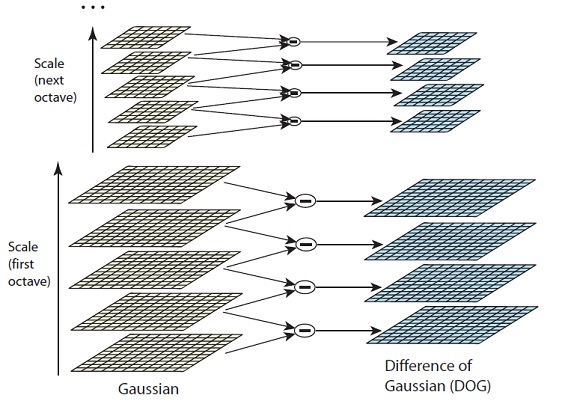
\includegraphics[width=0.65\textwidth]{fig/30.png}
     \vspace{-1em}
    \begin{center}    
       \caption{\textcolor{gray}{\footnotesize \textit{ }}}
    \label{fig:difference}
     \end{center}
     \vspace{-2.5em}
  \end{figure} \noindent
Når DoG billederne er blevet produceret, skal ekstremaer udvælges. Ekstremaer udvælges da de indikere at der opstår blobs. Da $DoG \approx LoG$, og $LoG$ svarer til sporret af hessian matricen, eller summen af egenværdierne :$$\Delta L = L{xx}+L_{yy} $$, vil der opstå et maksima når $\Delta L<0$, da egenværdierne begge vil være negative og et minima når $\Delta L > 0$ da egenværdierne vil være positive, hvor egenværdierne bestemmer den principielle krumning i og omkring et punkt og en krumning i hver sin retning vil indikere et saddle-point og derved ikke et ekstrema.
For hver pixel, sammenlignes et $3\times3\times3$ område, som vist figur \ref{fig:difference} b. Hver pixel bliver derved sammenlignet med dens 27 naboer i de omkringliggende DoG billeder, hvor punktet bliver udvalgt til et ekstrema, hvis det er det største/mindste iblandt de 27 naboer. 
\\
\\
Når lokale ekstremaer er udvalgt fravælges dårligt lokaliserede punkter, f.eks. ekstremaer med lav kontrast, men også punkter, hvor ekstremaer ligger imellem pixels. Ligeledes bliver punkters placering fundet, med subpixel nøjagtighed. Dette gøres, ved non-maximal suppression, som foreslået af Lowe \cite{nonmaximalsuppression}:
\begin{equation}
D(x)=D+\dfrac{\partial D^T}{\partial x}x\dfrac{1}{2}x^T\dfrac{\partial^2D}{\partial x^2}x
\label{nonmax}
\end{equation}
Ovenstående kan forstås om en Taylor udvidelse af i punket D.
Lokationen af ekstremaet $\hat{x}$ findes ved at tage den afledte af den ovenstående funktion ift. $x$ og sætte den til 0:
\begin{equation}
\hat{x}= \dfrac{\partial^2 D^{-1}}{\partial x^2}\dfrac{\partial D}{\partial x}
\end{equation}
Non-maximal suppression er blevet brugt anderledes i denne opgave, ifht. SIFT beskrivelsen: Lowe foreslår, at hvis et punkt er et ekstrema, som udregnet ved ligning\ref{nonmax} og $\hat{x} > 0.5$ i en retning, skal ligning \ref{nonmax} udregnes omkring det nye punkt og dette gentages, indtil $\hat{x} < 0.5$ (eller indtil udregning er udført et max antal gange).
\\
I denne opgave bliver et punkt fjernet, hvis $\hat{x} > 0.5$ i en given retning, da dette kun ville kunne øge antallet af interessepunkter, hvilket ikke er nødvendigt, da der er mange. Det vil ligeledes øge kompleksiteten af applikationen.
\\
Nu skal punkter med la kontrast fjernes, ved at sætte grænseværdi, for $D(\hat{x})$:
\begin{equation}
D(\hat{x})=D+\dfrac{1}{2}\dfrac{\partial D^T}{\partial x}\hat{x}
\end{equation}
Lowe foreslår at værdier af $D(\hat{x})$ under 0.03 fjernes. Metoden vil også have en positiv respons overfor kanter, derfor anvendes metoder lånt fra Harris og Stephens \cite{harris} til at fjerne disse. Hessian matricen opstilles som:
\begin{equation}
H =
\begin{bmatrix}
D_{xx} & D{xy} \\
D{xy} & D{yy}
\end{bmatrix}
\end{equation}
Hvor en grænseværdi for $r$ kan opstilles for at fjerne punkter lokaliseret på en kant:
\begin{equation}
\dfrac{tr(H)^2}{Det(H)}<\dfrac{(r+1)^2}{r}
\end{equation}
Punkter der tilfredsstiller denne grænseværdi udvælges som interessepunkter. 
\subsection*{Algoritme}
\begin{enumerate}
\item{Konstruer skalarummet for de forskellige oktaver, ved iterativt at folde skalabilledet med en stigende værdi af $\sigma$: $$ L(x,y,\sigma)= G(x,y,\sigma) \ast I(x,y) $$}
\item{Udregn "\textit{Difference of Gaussian}" billeder, ved at tage forskellen imellem skala billederne: $$ L(x,y,k \sigma)-L(x,y,\sigma)$$ }
\item{Lokaliser ekstremaer for hvert punkt i "\textit{Difference of Gaussian}" billeder, ved at sammenligne punktet med dens 27 naboer.}
\item{Afvis punkter der ikke er lokaliseret på ekstremaer, d.v.s. afvis punkter, der ikke opfylder følgende 
$$ \hat{x}<0.5 $$
Fjern punkter lokaliseret på ustabile ekstremaer ved at afvise punkter, der ikke opfylder:
$$ |D(\hat{x})|>0.03 $$}
\item{ Opstil Hessian matricen for at fjerne punkter lokaliseret på en kant: $$ \begin{bmatrix}
D_{xx} & D{xy} \\
D{xy} & D{yy}
\end{bmatrix} $$ 
og fjern punkter der ikke opfylder:
$$ \dfrac{tr(H)^2}{Det(H)}<\dfrac{(r+1)^2}{r}
$$
}
\end{enumerate}